% This is samplepaper.tex, a sample chapter demonstrating the
% LLNCS macro package for Springer Computer Science proceedings;
% Version 2.25 of 2026/09/03
%
\documentclass[runningheads]{llncs}
%
\usepackage[T1]{fontenc}
% T1 fonts will be used to generate the final print and online PDFs,
% so please use T1 fonts in your manuscript whenever possible.
% Other font encondings may result in incorrect characters.
%

\usepackage{mathptmx}       % selects Times Roman as basic font


\usepackage{graphicx}
% Used for displaying a sample figure. If possible, figure files should
% be included in EPS format.
%
% If you use the hyperref package, please uncomment the following two lines
% to display URLs in blue roman font according to Springer's eBook style:
%\usepackage{color}
%\renewcommand\UrlFont{\color{blue}\rmfamily}
%\urlstyle{rm}
%
\begin{document}
%
\title{Integrating Microclimate and Future Climate Scenarios in Urban Building Energy Modelling: Simulating Indoor Overheating, Energy Demand, and Prospective Life Cycle Assessment in Antwerp City, Belgium}
%
%\titlerunning{Abbreviated paper title}
% If the paper title is too long for the running head, you can set
% an abbreviated paper title here
%
\author{Richard Dean F. Morales\inst{1} \and
Dirk Lauwaet\inst{2} \and
Isabela Pichardo-Velázquez\inst{3,4} \and
\inst{3} \and
Yinthe Broeckx\inst{1} \and
Benjamin Lanssens\inst{2} \and
Amaryllis Audenaert\inst{1} \and
Antonino Marvuglia\inst{3} \and
Yixiao Ma\inst{2} \and
Stijn Verbeke\inst{1,2,5}} 
%
\authorrunning{F. Author et al.}
% First names are abbreviated in the running head.
% If there are more than two authors, 'et al.' is used.
%
\institute{University of Antwerp, Antwerp, Belgium \and
Flemish Insititute for Technological Research (VITO), Mol, Belgium \and
Luxembourg Insititute of Science and Technology \and
University of Luxembourg, Luxembourg \and
EnergyVille, Genk, Belgium}
%
\maketitle              % typeset the header of the contribution
%
\begin{abstract}
The compounding impacts of the Urban Heat Island (UHI) effect and climate change pose severe risks to the thermal resilience of dense urban environments. Standard building performance simulations relying on macro-scale historic weather data frequently underestimate localized thermal loads and subsequent indoor overheating. This study presents an innovative Urban Building Energy Modelling (UBEM) framework applied to the historic city center of Antwerp, utilizing Level of Detail 2 (LoD 2) building geometries to simulate localized microclimates while simultaneously projecting performance into future climate horizons. By integrating high-resolution microclimate data, the model explicitly captures district-specific thermal intensification compared to standard historic weather baselines. Preliminary results quantify this impact, revealing that microclimatic UHI effects increase indoor overheating hours by 21\% while concurrently reducing annual heating demand by 10\% compared to historic weather datasets. To evaluate long-term mitigation and adaptation pathways and account for the environmental cost of necessary physical interventions, the study incorporates building stock transition scenarios projected under distinct future climate pathways, specifically contrasting the low-emission SSP1-2.6 and high-emission SSP3-7.0 scenarios. Under these future horizons, microclimatic compounding is expected to further escalate indoor heat vulnerability. A comprehensive Life Cycle Assessment (LCA) of the district is integrated into the methodology for a robust evaluation of shifting heating energy demands and overheating risks. The LCA highlights the environmental trade-offs of the required urban transition strategies, contrasting the initial embodied carbon of necessary structural interventions against their long-term operational emission savings across different climate realities. This research demonstrates the necessity of coupling high-detail geometric modelling with aligned future weather, microclimate, and lifecycle transition projections to accurately inform the climate-proofing of cities.

\keywords{Microclimate  \and Future Climate \and Urban Building Energy Modelling \and Urban Building Comfort Modelling \and Life Cycle Assessment}
\end{abstract}
%
%
%
\section{First Section}
\subsection{A Subsection Sample}
Please note that the first paragraph of a section or subsection is
not indented. The first paragraph that follows a table, figure,
equation etc. does not need an indent, either.

Subsequent paragraphs, however, are indented.

\subsubsection{Sample Heading (Third Level)} Only two levels of
headings should be numbered. Lower level headings remain unnumbered;
they are formatted as run-in headings.

\paragraph{Sample Heading (Fourth Level)}
The contribution should contain no more than four levels of
headings. Table~\ref{tab1} gives a summary of all heading levels.

\begin{table}
\caption{Table captions should be placed above the
tables.}\label{tab1}
\begin{tabular}{|l|l|l|}
\hline
Heading level &  Example & Font size and style\\
\hline
Title (centered) &  {\Large\bfseries Lecture Notes} & 14 point, bold\\
1st-level heading &  {\large\bfseries 1 Introduction} & 12 point, bold\\
2nd-level heading & {\bfseries 2.1 Printing Area} & 10 point, bold\\
3rd-level heading & {\bfseries Run-in Heading in Bold.} Text follows & 10 point, bold\\
4th-level heading & {\itshape Lowest Level Heading.} Text follows & 10 point, italic\\
\hline
\end{tabular}
\end{table}


\noindent Displayed equations are centered and set on a separate
line.
\begin{equation}
x + y = z
\end{equation}
Please try to avoid rasterized images for line-art diagrams and
schemas. Whenever possible, use vector graphics instead (see
Fig.~\ref{fig1}).

\begin{figure}
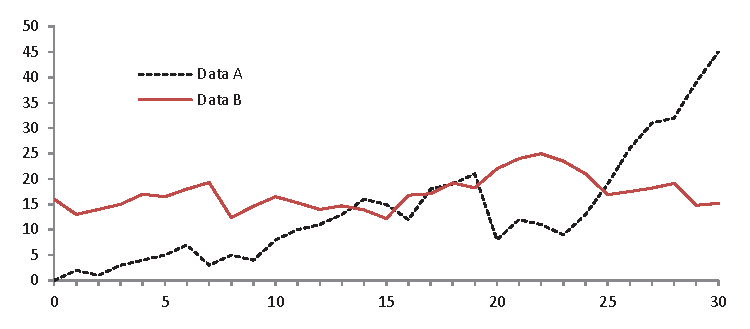
\includegraphics[width=\textwidth]{figures/fig1}
\Description{In LaTeX you may insert your alternative texts into your manuscript using the \verb|\Description| command in a \verb|figure| environment}
\caption{A figure caption is always placed below the illustration.
Please note that short captions are centered, while long ones are
justified by the macro package automatically.} \label{fig1}
\end{figure}

\begin{theorem}
This is a sample theorem. The run-in heading is set in bold, while
the following text appears in italics. Definitions, lemmas,
propositions, and corollaries are styled the same way.
\end{theorem}
%
% the environments 'definition', 'lemma', 'proposition', 'corollary',
% 'remark', and 'example' are defined in the LLNCS documentclass as well.
%
\begin{proof}
Proofs, examples, and remarks have the initial word in italics,
while the following text appears in normal font.
\end{proof}
For citations of references, we prefer the use of square brackets
and consecutive numbers. Citations using labels or the author/year
convention are also acceptable. The following bibliography provides
a sample reference list with entries for journal
articles~\cite{ref_article1}, an LNCS chapter~\cite{ref_lncs1}, a
book~\cite{ref_book1}, proceedings without editors~\cite{ref_proc1},
and a homepage~\cite{ref_url1}. Multiple citations are grouped
\cite{ref_article1,ref_lncs1,ref_book1},
\cite{ref_article1,ref_book1,ref_proc1,ref_url1}.

\begin{credits}
\subsubsection{\ackname} A bold run-in heading in small font size at the end of the paper is
used for general acknowledgments, for example: This study was funded
by X (grant number Y).

\subsubsection{\discintname}
It is now necessary to declare any competing interests or to specifically
state that the authors have no competing interests. Please place the
statement with a bold run-in heading in small font size beneath the
(optional) acknowledgments\footnote{If EquinOCS, our proceedings submission
system, is used, then the disclaimer can be provided directly in the system.},
for example: The authors have no competing interests to declare that are
relevant to the content of this article. Or: Author A has received research
grants from Company W. Author B has received a speaker honorarium from
Company X and owns stock in Company Y. Author C is a member of committee Z.
\end{credits}
%
% ---- Bibliography ----
%
% BibTeX users should specify bibliography style 'splncs04'.
% References will then be sorted and formatted in the correct style.
%
% \bibliographystyle{splncs04}
% \bibliography{mybibliography}
%
\begin{thebibliography}{8}
\bibitem{ref_article1}
Author, F.: Article title. Journal \textbf{2}(5), 99--110 (2016)

\bibitem{ref_lncs1}
Author, F., Author, S.: Title of a proceedings paper. In: Editor,
F., Editor, S. (eds.) CONFERENCE 2016, LNCS, vol. 9999, pp. 1--13.
Springer, Heidelberg (2016). \doi{10.10007/1234567890}

\bibitem{ref_book1}
Author, F., Author, S., Author, T.: Book title. 2nd edn. Publisher,
Location (1999)

\bibitem{ref_proc1}
Author, A.-B.: Contribution title. In: 9th International Proceedings
on Proceedings, pp. 1--2. Publisher, Location (2010)

\bibitem{ref_url1}
LNCS Homepage, \url{http://www.springer.com/lncs}, last accessed 2023/10/25
\end{thebibliography}
\end{document}
